% ArtiGate-YOLO - main manuscript prototype.
%
% This file compiles with the standard IEEEtran journal class so the draft can be built anywhere.
% For submission, move the content into the official IEEE Access LaTeX template
% (https://ieeeaccess.ieee.org/authors/preparing-your-article/ or the "IEEE Access LaTeX Template" on
% Overleaf): keep its front matter (\history, \doi, \address, \corresp, \tfootnote, \EOD) and
% \input the same files from sections/. See paper/README.md.
%
% Every value that does not exist yet is written as \TBD{...} (red in the PDF). No result in this
% draft is real; fill them from runs/ only.

\documentclass[journal]{IEEEtran}
\usepackage{amsmath,amssymb}
\usepackage{graphicx}
\usepackage{booktabs}
\usepackage{multirow}
\usepackage{array}
\usepackage{tabularx}
\usepackage{subcaption}
\usepackage{tikz}
\usetikzlibrary{arrows.meta,positioning,fit,calc,backgrounds}
\usepackage[hidelinks]{hyperref}
% Shared macros for the main manuscript and the Supplementary Material.
\usepackage{xcolor}
% \TBD{...} marks every value that does not exist yet (results, decisions, citations to check).
% Search the .tex files for "\TBD" before submission; the PDF shows them in red.
\newcommand{\TBD}[1]{\textcolor{red}{[#1]}}
\newcommand{\res}{\TBD{--}} % one result cell that the experiments will fill
\newcommand{\etal}{\textit{et~al.}}
\newcommand{\method}{ArtiGate-YOLO}
\newcommand{\aga}{AGA}
\newcommand{\Abar}{\bar{A}}
% Placeholder for a figure that will be produced from the runs.
\newcommand{\placeholderfig}[2]{%
  \fbox{\parbox[c][#1][c]{0.94\linewidth}{\centering\small\textcolor{red}{#2}}}}


\begin{document}

\title{ArtiGate-YOLO: Artifact-Supervised Gated Attention for Robust Real-Time Skin Lesion Segmentation}

\author{\TBD{Author 1},~\TBD{Author 2}%
\thanks{\TBD{Affiliation, address, e-mail, funding. Corresponding author.}}}

\markboth{IEEE Access (draft)}{\TBD{Authors}: ArtiGate-YOLO}

\maketitle

% IEEE Access: one paragraph, about 150-250 words, no citations. Rewrite the result sentences once
% the numbers exist; keep only claims the results support.
\begin{abstract}
Hair, ruler markings, surgical ink and dark vignette corners are common in dermoscopic images and are a known source of segmentation errors and shortcut learning. Existing remedies either remove artifacts before segmentation, estimate them with hand-set rules, or learn an artifact map without supervision. We propose ArtiGate-YOLO, a real-time instance segmentation model that learns where artifacts are and uses that knowledge inside the network. A lightweight artifact head on the stride-4 backbone features predicts four artifact maps (hair, ruler, marker ink, dark corner). It is supervised with pixel-exact masks of procedurally composited artifacts and with partial labels, so no artifact is annotated by hand at the pixel level. The resulting map drives Artifact-Gated Attention (AGA), a drop-in replacement for CBAM whose spatial attention receives the artifact map and whose output is attenuated where artifacts are predicted; at initialization AGA is identical to CBAM. The model adds 0.021~M parameters and 1.05~GFLOPs at $640\times640$ to a YOLO26n-seg baseline with a P2 head and CBAM and needs a single RGB image at inference. On ISIC~2018 Task~1, ArtiGate-YOLO reaches a Dice score of \TBD{x.xxx} against \TBD{x.xxx} for the same network with CBAM, with \TBD{the largest gains on images that contain hair or rulers} and \TBD{no loss on artifact-free images}. Under synthetic artifacts of increasing severity, \TBD{its Dice decreases by x.x points against y.y}, and on the external PH2 set it reaches \TBD{x.xxx}. Code, trained models and the artifact annotations of the test set will be released.
\end{abstract}

\begin{IEEEkeywords}
Dermoscopy, skin lesion segmentation, imaging artifacts, attention, YOLO, robustness, synthetic data, partial labels.
\end{IEEEkeywords}


\section{Introduction}\label{sec:intro}
Segmenting the lesion is the first step of most computer-aided dermoscopy pipelines: the mask defines the region from which border irregularity, asymmetry and colour variegation are measured, and it restricts classifiers to the lesion~\cite{mirikharaji2023survey}. Dermoscopic images, however, rarely show only skin and lesion. Terminal hairs cross the lesion border, rulers and calibration marks lie along the image edge, surgeons draw ink circles around suspicious lesions, and the circular aperture of the dermatoscope leaves dark corners. These structures are dark, thin or high-contrast, and they resemble lesion boundaries closely enough to pull a segmentation network away from the true contour. They also carry dataset-specific correlations: surgical skin markings were associated with altered melanoma predictions of a convolutional classifier~\cite{winkler2019markings}, and models trained on ISIC data can exploit artifacts as shortcuts~\cite{bissoto2020debiasing,geirhos2020shortcut}.

Three families of remedies exist. The oldest removes hair before analysis with morphological filtering and inpainting, as in DullRazor~\cite{lee1997dullrazor,telea2004inpainting}; such preprocessing is tuned by hand, handles one artifact type, and may erase genuine dark structures inside the lesion. Detection pipelines still apply it as a separate step~\cite{rana2025explainable}. A second family builds an artifact estimate into the network with fixed rules: FSSM-ResNet scores hair-like pixels by darkness, thinness and linearity in a fuzzy module and suppresses them during decoding~\cite{raikhankyzy2026fssm}. A third family learns the estimate end to end without artifact labels, either as a confidence map that scales a residual stream~\cite{singh2025dualresolution} or as multi-cue artifact responses that gate skip connections~\cite{gong2026artifactaware}. None of these methods tells the network which pixels are artifacts and of which type; the artifact map is either hand-crafted or left to emerge from the segmentation loss.

Supervising an artifact map directly has been impractical because pixel-level artifact annotations are scarce. Image-level artifact labels exist for the ISIC 2018 training set~\cite{bissoto2020debiasing,bissoto2022artifact}, a hair-mask set covers 500 images~\cite{hossain2023hairmask}, and marker and ruler masks exist for a small clinical set~\cite{carrion2023fedd}. Recent simulators show that artifacts can instead be generated with exact masks~\cite{kim2024ssynth,sizikova2026oasis}. We follow that route and combine it with partial labels: synthetic artifacts provide positives with exact masks, image-level labels and conservative colour and morphology rules provide negatives, and every remaining pixel is ignored by the loss.

This paper presents ArtiGate-YOLO, built on YOLO26n-seg~\cite{jocher2026yolo26} with an additional P2 detection level for small structures. Our earlier conference model added CBAM~\cite{woo2018cbam} to the stride-4 and stride-8 backbone features~\cite{iceeis2026own}; ArtiGate-YOLO keeps that network and changes only how attention is computed. The contributions are:
\begin{enumerate}
  \item An artifact head inside a real-time YOLO segmentation network that predicts four artifact types (hair, ruler, marker ink, dark corner) at stride~4 and is trained without manual artifact annotation, through procedurally composited artifacts with pixel-exact masks and a partial-label loss.
  \item Artifact-Gated Attention (AGA), a drop-in replacement for CBAM whose spatial attention receives the predicted artifact map and whose output is attenuated where artifacts are predicted. AGA reduces exactly to CBAM at initialization, and control rows separate the effects of training on artifact-augmented images, of the auxiliary artifact task and of gating with a supervised rather than an unsupervised map.
  \item A robustness evaluation by artifact type and severity: results stratified by artifact presence on the ISIC 2018 test set (image-level labels we release), a severity sweep with held-out synthetic artifacts, external validation on three test sets, and a test of the artifact maps against real marker, ruler and hair masks that were never used for training, all with image-level paired statistics over three training seeds.
\end{enumerate}

Section~\ref{sec:related} reviews related work, Section~\ref{sec:method} describes the model and its training targets, Section~\ref{sec:protocol} the datasets, baselines and statistical protocol, and Section~\ref{sec:results} the results. Section~\ref{sec:discussion} discusses limitations, and Section~\ref{sec:conclusion} concludes. The Supplementary Material holds the complete tables, the generator parameters and implementation details.


\section{Related Work}\label{sec:related}
\subsection{Skin Lesion Segmentation}
Encoder-decoder networks derived from U-Net~\cite{ronneberger2015unet} dominate dermoscopic lesion segmentation, and the self-configuring nnU-Net~\cite{isensee2021nnunet} is a strong general-purpose reference; a recent survey covers the field~\cite{mirikharaji2023survey}. For deployment on limited hardware, lightweight variants such as MALUNet~\cite{ruan2022malunet} and EGE-UNet~\cite{ruan2023egeunet} reduce parameters and computation. Single-stage instance segmentation models of the YOLO family offer real-time inference and a mature training pipeline with strong augmentation~\cite{bochkovskiy2020yolov4,jocher2026yolo26}; YOLO26 removes non-maximum suppression and predicts masks from prototypes. \TBD{Add 2--3 recent YOLO-based lesion segmentation papers after the October 2026 literature check.}

\subsection{Artifacts and Shortcut Learning in Dermoscopy}
Bissoto~\etal\ annotated seven artifact types (dark corners, hair, gel borders, gel bubbles, rulers, ink markings and patches) on the ISIC 2018 training images and showed that classifiers exploit them~\cite{bissoto2020debiasing,bissoto2022artifact}; the labels were later used for artifact-based domain generalization~\cite{bissoto2022artifact}. Surgical ink markings changed the outputs of a melanoma classifier~\cite{winkler2019markings}. These findings are instances of shortcut learning~\cite{geirhos2020shortcut}. For segmentation, the usual response is hair removal before training or inference~\cite{lee1997dullrazor,rana2025explainable}.

Closest to our work are methods that handle artifacts inside the network. FSSM-ResNet embeds a fuzzy structural suppression module that scores hair-like pixels by darkness, thinness and linearity and suppresses them during decoding~\cite{raikhankyzy2026fssm}. A dual-resolution residual network predicts a per-pixel artifact confidence map with a shallow head and uses it, with a learned strength, to scale the residual stream; the head receives no direct supervision~\cite{singh2025dualresolution}. An artifact-aware lightweight segmenter combines Laplacian, bright-region, dark-region and learned responses in a multi-cue stem and gates the skip connections with the propagated artifact cues~\cite{gong2026artifactaware}. Table~\ref{tab:related} contrasts these designs with ours: none supervises the artifact map with artifact masks, none separates artifact types, and none is a real-time YOLO-style model.

\begin{table}[!t]
\centering
\caption{Methods that handle dermoscopic artifacts inside or before the segmentation network.}
\label{tab:related}
\footnotesize
\setlength{\tabcolsep}{3pt}
\begin{tabularx}{\columnwidth}{@{}>{\raggedright\arraybackslash}p{0.21\columnwidth}>{\raggedright\arraybackslash}X>{\raggedright\arraybackslash}p{0.14\columnwidth}>{\raggedright\arraybackslash}p{0.15\columnwidth}@{}}
\toprule
Method & Artifact estimate & Types & Supervised map \\
\midrule
DullRazor~\cite{lee1997dullrazor} & Morphological filter + inpainting before the model & Hair & No (rules) \\
YOLO + hair removal~\cite{rana2025explainable} & Separate preprocessing step & Hair & No (rules) \\
FSSM-ResNet~\cite{raikhankyzy2026fssm} & Embedded fuzzy hair score, suppression in decoder & Hair & No (rules) \\
Dual-resolution~\cite{singh2025dualresolution} & Shallow confidence head scales residual stream & Unspecified & No \\
Artifact-aware~\cite{gong2026artifactaware} & Multi-cue stem, gated skip fusion & Unspecified & No \\
\textbf{Ours} & Artifact head on stride-4 features, gates attention & 4 & Yes (synthetic + partial) \\
\bottomrule
\end{tabularx}
\end{table}

\subsection{Attention and Auxiliary Supervision}
Squeeze-and-excitation~\cite{hu2018senet} and CBAM~\cite{woo2018cbam} reweight channels and spatial positions from pooled feature statistics. Their spatial attention is computed from the features alone, so nothing tells it which bright or dark structures are irrelevant. Auxiliary tasks can shape shared representations~\cite{caruana1997multitask}; in our ablation, an artifact head trained only as an auxiliary task (row A2) separates this multi-task effect from the effect of feeding the artifact map into attention (row A4).

\subsection{Synthetic Artifacts and Robustness Evaluation}
Physics- and knowledge-based simulators generate skin images with exact masks: S-SYNTH models skin layers, lesions and hair~\cite{kim2024ssynth}, and OASIS adds rulers, calibration charts, hair and vessels with pixel-level masks and artifact-free counterparts~\cite{sizikova2026oasis}. Corruption benchmarks quantify robustness by severity level~\cite{hendrycks2019benchmarking}. We use procedural compositing on real dermoscopic images both to supervise the artifact head and to build a severity sweep; because a generator shared by training and testing can overstate robustness, our main robustness claims rest on real artifacts (Section~\ref{sec:protocol}).


\section{Method}\label{sec:method}
\begin{figure*}[!t]
\centering
% Fig. 1: ArtiGate-YOLO overview (top) and the AGA block (bottom). TikZ, no external files.
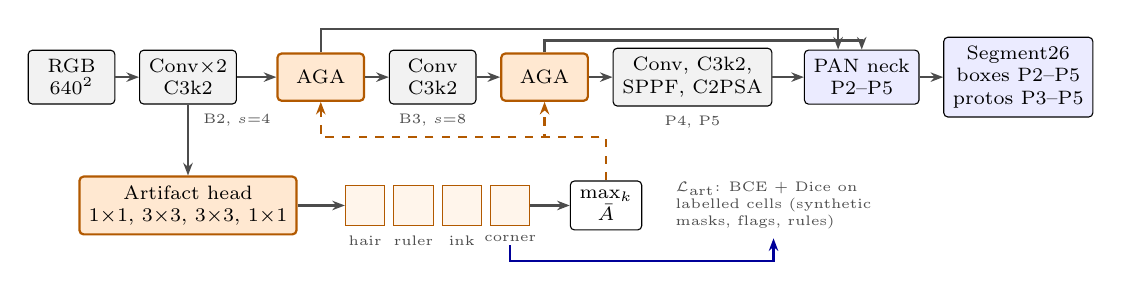
\begin{tikzpicture}[
  font=\scriptsize,
  >={Stealth[length=1.6mm]},
  blk/.style={draw, rounded corners=1.5pt, minimum height=6mm, minimum width=11mm, align=center, fill=white},
  bb/.style={blk, fill=gray!10},
  new/.style={blk, fill=orange!18, draw=orange!70!black, thick},
  head/.style={blk, fill=blue!8},
  map/.style={draw=orange!70!black, fill=orange!8, minimum size=5mm, inner sep=0pt},
  lab/.style={font=\tiny, text=black!70},
  line/.style={->, thick, black!70},
  aline/.style={->, thick, orange!70!black, dashed},
]
% ---------------------------------------------------------------- backbone row
\node[bb] (in) {RGB\\$640^2$};
\node[bb, right=3mm of in] (c0) {Conv$\times$2\\C3k2};
\node[lab, anchor=north west] at ($(c0.south)+(0.7mm,0)$) {B2, $s{=}4$};
\node[new, right=5mm of c0] (aga2) {AGA};
\node[bb, right=3mm of aga2] (c1) {Conv\\C3k2};
\node[lab, below=0mm of c1] {B3, $s{=}8$};
\node[new, right=3mm of c1] (aga3) {AGA};
\node[bb, right=3mm of aga3] (c2) {Conv, C3k2,\\SPPF, C2PSA};
\node[lab, below=0mm of c2] {P4, P5};
\node[head, right=4mm of c2] (neck) {PAN neck\\P2--P5};
\node[head, right=3mm of neck] (seg) {Segment26\\boxes P2--P5\\protos P3--P5};
\draw[line] (in) -- (c0);
\draw[line] (c0) -- (aga2);
\draw[line] (aga2) -- (c1);
\draw[line] (c1) -- (aga3);
\draw[line] (aga3) -- (c2);
\draw[line] (c2) -- (neck);
\draw[line] (neck) -- (seg);
\draw[line] (aga2.north) -- ++(0,3mm) -| ($(neck.north)+(-3mm,0)$);
\draw[line] (aga3.north) -- ++(0,1.5mm) -| ($(neck.north)+(0mm,0)$);
% ---------------------------------------------------------------- artifact head
\node[new, below=9mm of c0] (ah) {Artifact head\\$1{\times}1$, $3{\times}3$, $3{\times}3$, $1{\times}1$};
\draw[line] (c0.south) -- (ah.north);
\node[map, right=6mm of ah, label={[lab]below:hair}] (m1) {};
\node[map, right=1mm of m1, label={[lab]below:ruler}] (m2) {};
\node[map, right=1mm of m2, label={[lab]below:ink}] (m3) {};
\node[map, right=1mm of m3, label={[lab]below:corner}] (m4) {};
\node[fit=(m1)(m4), inner sep=1pt] (maps) {};
\draw[line] (ah) -- (m1);
\node[blk, right=5mm of m4, minimum width=9mm] (amax) {$\max_k$\\$\bar{A}$};
\draw[line] (m4) -- (amax);
\draw[aline] (amax.north) |- ($(aga2.south)+(0,-4.5mm)$) -- (aga2.south);
\draw[aline] (amax.north) |- ($(aga3.south)+(0,-4.5mm)$) -- (aga3.south);
\node[lab, align=left, right=3mm of amax] (loss) {$\mathcal{L}_{\mathrm{art}}$: BCE + Dice on\\labelled cells (synthetic\\masks, flags, rules)};
\draw[->, thick, blue!60!black] ($(m4.south)+(0,-2.5mm)$) -- ++(0,-2mm) -| (loss.south);
\end{tikzpicture}

\vspace{2mm}
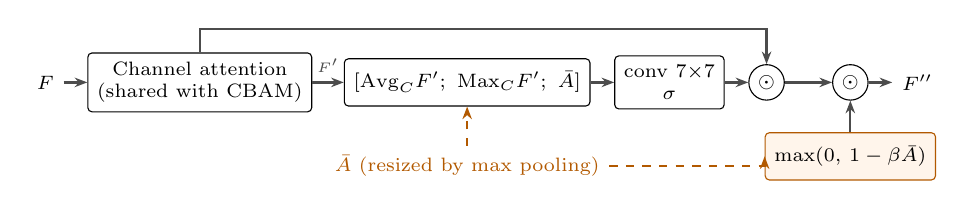
\begin{tikzpicture}[
  font=\scriptsize,
  >={Stealth[length=1.6mm]},
  blk/.style={draw, rounded corners=1.5pt, minimum height=6mm, align=center, fill=white},
  op/.style={draw, circle, inner sep=0.5pt, minimum size=4.5mm},
  line/.style={->, thick, black!70},
  aline/.style={->, thick, orange!70!black, dashed},
]
\node (F) {$F$};
\node[blk, right=3mm of F] (ca) {Channel attention\\(shared with CBAM)};
\node[blk, right=4mm of ca] (pool) {$[\mathrm{Avg}_C F';\ \mathrm{Max}_C F';\ \bar{A}]$};
\node[blk, right=3mm of pool] (conv) {conv $7{\times}7$\\$\sigma$};
\node[op, right=3mm of conv] (mul1) {$\odot$};
\node[op, right=6mm of mul1] (mul2) {$\odot$};
\node[right=3mm of mul2] (out) {$F''$};
\node[blk, below=4mm of mul2, fill=orange!8, draw=orange!70!black] (gate) {$\max(0,\,1-\beta\bar{A})$};
\node[below=5mm of pool, text=orange!70!black] (A) {$\bar{A}$ (resized by max pooling)};
\draw[line] (F) -- (ca);
\draw[line] (ca) -- node[above, font=\tiny]{$F'$} (pool);
\draw[line] (pool) -- (conv);
\draw[line] (conv) -- (mul1);
\draw[line] (mul1) -- (mul2);
\draw[line] (mul2) -- (out);
\draw[line] (ca.north) -- ++(0,3mm) -| (mul1.north);
\draw[aline] (A.north) -- (pool.south);
\draw[aline] (A.east) -| (gate.west) ;
\draw[line] (gate) -- (mul2);
\end{tikzpicture}

\caption{ArtiGate-YOLO. Top: the artifact head reads the stride-4 backbone feature B2 and predicts four artifact maps; their pixel-wise maximum $\bar{A}$ is passed to the two AGA blocks that replace CBAM after B2 and B3. The rest is YOLO26n-seg with a P2 detection level; mask prototypes are built from P3--P5 at stride~4. Bottom: the AGA block. Its channel attention is the CBAM channel attention; the spatial attention receives $\bar{A}$ as a third input and the output is multiplied by $\max(0,1-\beta\bar{A})$. The weights on $\bar{A}$ and $\beta$ start at zero, so AGA equals CBAM at initialization. Dashed: artifact map; by default it is detached, so the segmentation loss does not train the artifact head.}
\label{fig:overview}
\end{figure*}

\subsection{Base Network}
The base network is YOLO26n-seg~\cite{jocher2026yolo26} with an additional P2 output, so boxes and mask coefficients are predicted at strides 4, 8, 16 and 32. Mask prototypes are computed from P3--P5 and upsampled once, which keeps them at stride~4. The CBAM baseline of our conference paper~\cite{iceeis2026own} (row A1 in Section~\ref{sec:protocol}) inserts CBAM~\cite{woo2018cbam} directly after the stride-4 feature B2 and the stride-8 feature B3 of the backbone. ArtiGate-YOLO keeps this network and replaces the two CBAM blocks with AGA blocks fed by an artifact head (Fig.~\ref{fig:overview}).

\subsection{Artifact Head}
Let $B_2\in\mathbb{R}^{C_2\times H/4\times W/4}$ be the B2 feature map ($C_2=64$ at scale n). The artifact head reduces it with a $1\times1$ convolution to $c_h=32$ channels, refines it with two $3\times3$ convolutions (these three convolutions are each followed by batch normalization and SiLU) and maps it with a plain $1\times1$ convolution to $K=4$ logits $Z\in\mathbb{R}^{K\times H/4\times W/4}$ for hair, ruler, marker ink and dark corner. The artifact probabilities are $A_k=\sigma(Z_k)$. The bias of the last layer is initialized to $\log(\pi/(1-\pi))$ with $\pi=0.01$ because artifacts cover few pixels. The combined map is the pixel-wise maximum over types,
\begin{equation}
\bar{A}=\max_{k=1,\dots,K} A_k ,
\label{eq:abar}
\end{equation}
computed from detached logits by default, so that the segmentation loss cannot push the head towards maps that hide the lesion; the head is then trained only by its own loss (Section~\ref{sec:loss}). Together with the two AGA blocks, the head adds about 21 thousand parameters (0.8\% of the deployed model) and 1.05~GFLOPs at $640\times640$ input (Supplementary Section~S10).

\subsection{Artifact-Gated Attention}
Given a feature map $F\in\mathbb{R}^{C\times H'\times W'}$ at the position of a CBAM block, AGA first applies the CBAM channel attention,
\begin{equation}
F'=\sigma\big(\mathrm{MLP}(\mathrm{Avg}_{HW}F)+\mathrm{MLP}(\mathrm{Max}_{HW}F)\big)\odot F,
\label{eq:ca}
\end{equation}
with a shared two-layer MLP (reduction 16, no bias). The artifact map is resized to $H'\times W'$ by max pooling, which keeps thin hairs visible at stride 8, giving $\bar{A}'$. The spatial attention and the gate are
\begin{equation}
\begin{aligned}
F''={}&F'\odot\sigma\Big(f^{7\times7}\big([\mathrm{Avg}_C F';\,\mathrm{Max}_C F';\,\bar{A}']\big)\Big)\\
&\odot\max\big(0,\,1-\beta\bar{A}'\big),
\end{aligned}
\label{eq:aga}
\end{equation}
where $f^{7\times7}$ is a $7\times7$ convolution with three input channels and $\beta$ is a learned scalar. The weights of $f^{7\times7}$ on the $\bar{A}'$ channel and $\beta$ are initialized to zero, so at initialization \eqref{eq:aga} reduces exactly to CBAM, and AGA departs from CBAM only as far as training moves these parameters away from zero. $\beta$ is not clamped: with a clamp to $[0,1]$, a $\beta$ that drifts below zero receives no gradient and stays there, which we observed in a development run. A positive $\beta$ attenuates features where artifacts are predicted and a negative $\beta$ would amplify them; weight decay pulls $\beta$ towards zero, that is, towards CBAM. We report the learned $\beta$ of each block.

\subsection{Training Targets Without Manual Annotation}\label{sec:targets}
\paragraph{Synthetic artifacts}
During training, each image receives procedurally drawn artifacts with probability $p_{\mathrm{synth}}=0.7$. Each of the four types is drawn independently (probabilities 0.5 for hair and 0.3 for the others, at least one type per image) with a severity sampled uniformly from $\{1,2,3,4\}$. Hair strands are cubic B\'ezier curves of random length, curvature, width and colour; rulers are light (occasionally dark) bands with tick marks and numerals along one image border, or two borders at the highest severity; marker ink forms dots, arcs or strokes around the lesion in purple, blue or black; dark corners are a circular dermatoscope aperture with a soft edge. The drawing order follows the physical layering (ink, hair, ruler, aperture). Rulers and marks never overlap the lesion bounding box and the aperture always contains it; only hair may cross the lesion, whose mask is unchanged. Every drawn artifact yields an exact mask, and the anti-aliased edge around it is marked as unknown; a later layer can cover an earlier one (for example, the aperture over hair), and the earlier mask is kept. Artifacts are drawn inside the image content area only, never on letterbox padding. The full parameter table is in Supplementary Section~S3, and examples are shown in Fig.~\ref{fig:synthetic}.

\paragraph{Partial labels}
For each artifact type a pixel is \emph{present}, \emph{absent} or \emph{unknown}. Synthetic artifacts give present pixels. Absent pixels come from two sources: image-level labels of the ISIC 2018 training images~\cite{bissoto2020debiasing,bissoto2022artifact}, which mark every pixel of an image as absent for the types it does not contain, and conservative rules that only exclude pixels which cannot show the artifact (for example, no hair where the morphological black-hat response is low, no dark corner where the brightness is at least 70; Supplementary Section~S4). All remaining pixels are unknown and do not contribute to the loss. Without the absent pixels the head would admit the trivial solution of predicting artifacts everywhere.

\paragraph{Joint augmentation}
The four target maps are stored as extra image channels (255 present, 0 absent, 114 unknown) and pass through the standard Ultralytics augmentation together with the image: mosaic, rotation, scaling, flips, mix-up and copy-paste. The maps therefore stay aligned with the image without changes to the augmentation code; after interpolation, a value of at least $0.75\cdot255$ counts as present, a value of at most $0.1\cdot255$ as absent and anything in between as unknown, so that mix-up of an absent with an unknown pixel stays unknown, and padding added by the augmentations is coded as unknown or absent, both correct because padding contains no artifact. Colour augmentation is applied to the image channels only, and the maps are split off before the forward pass.

\begin{figure*}[!t]
\centering
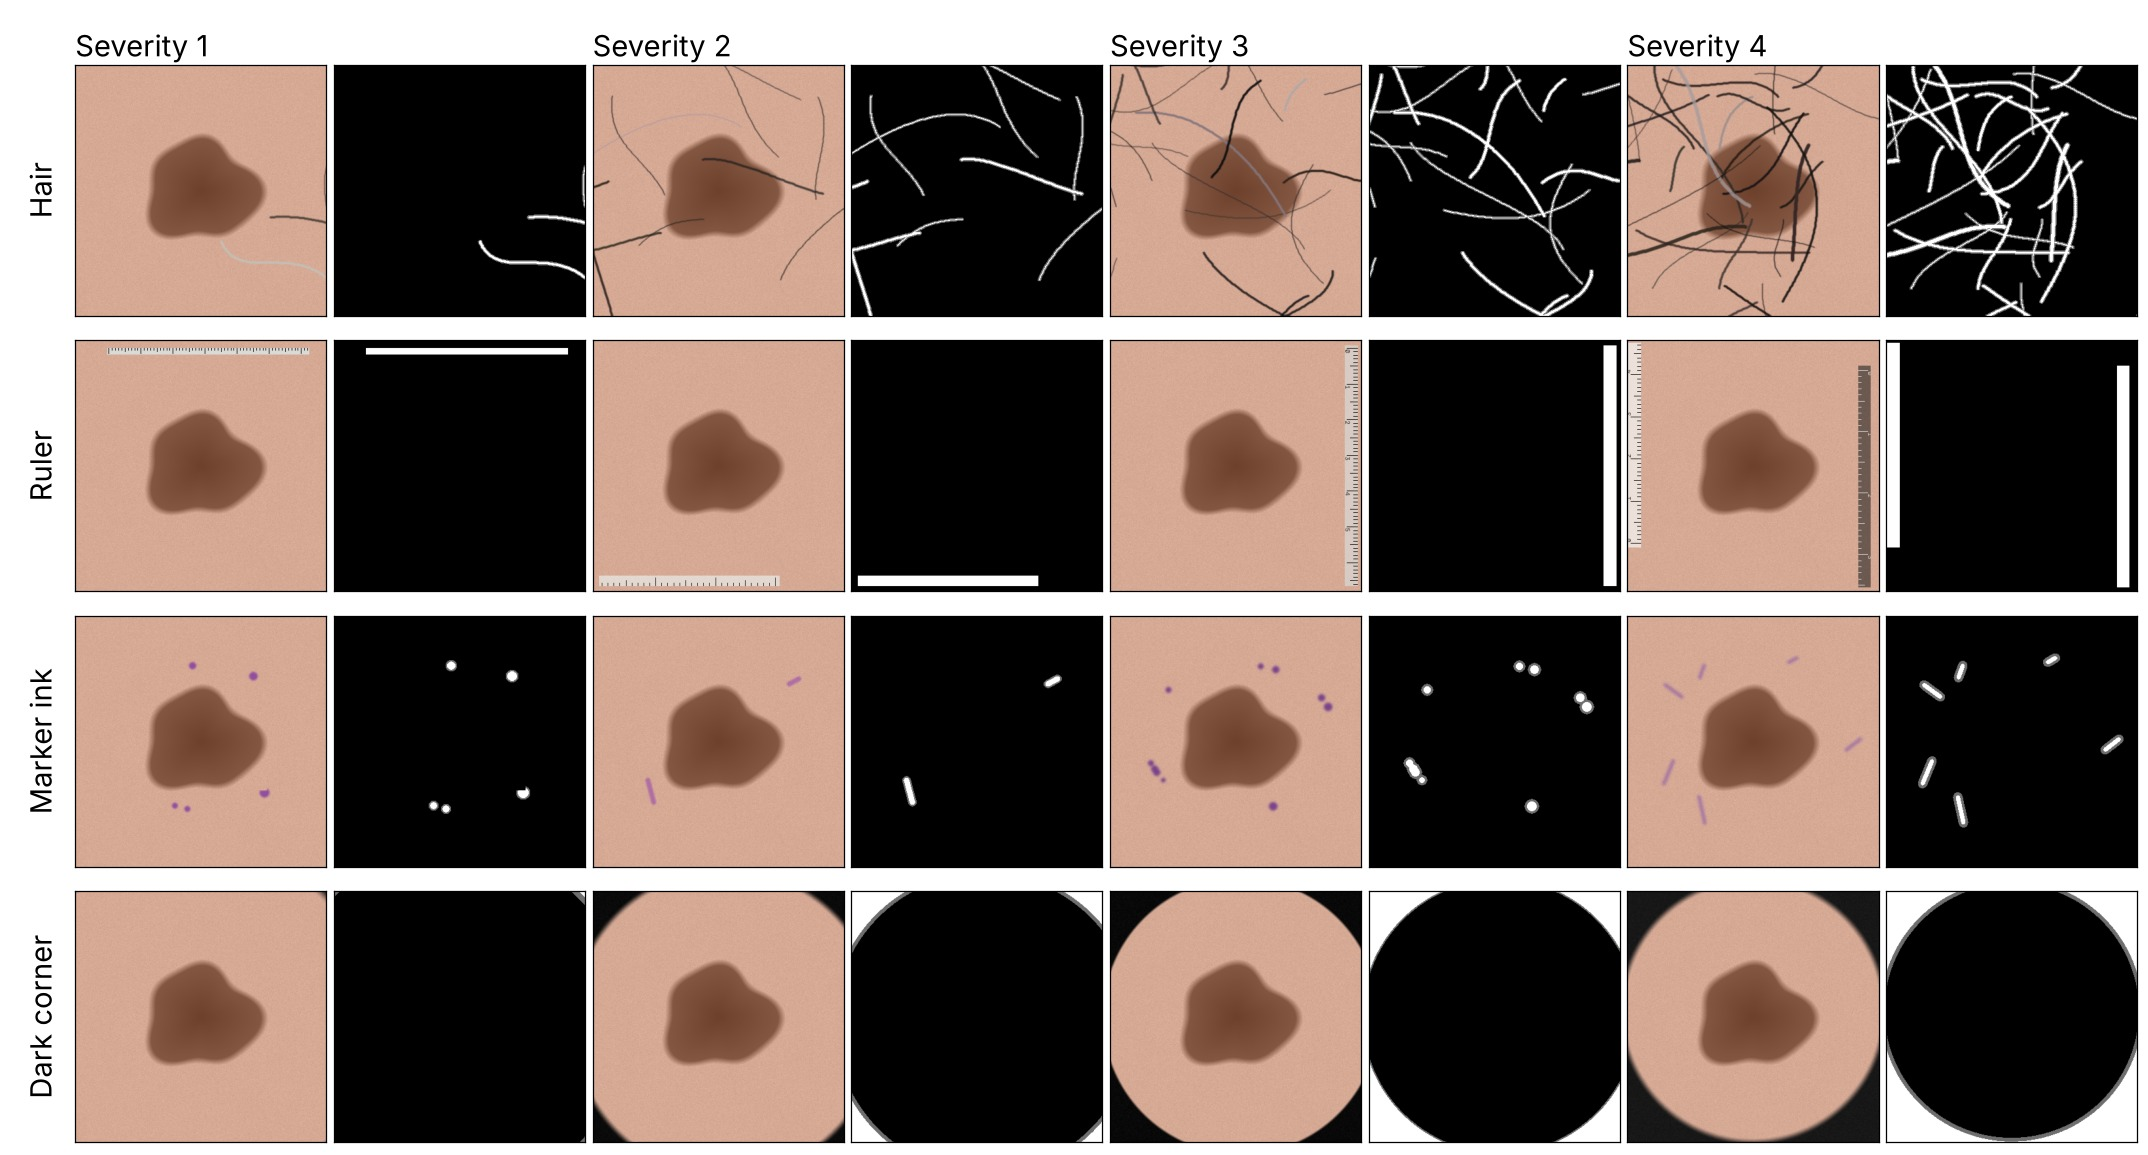
\includegraphics[width=\textwidth]{figures/synthetic_artifacts.jpg}
\caption{Procedural artifacts at severities 1--4 for hair, ruler, marker ink and dark corner (rows). Each severity shows the image and the training target of that type: white, present; grey, pixels changed by the artifact but outside its label (unknown); black, not changed by the generator (absent or unknown, depending on the image-level labels and rules). At severity~1 the aperture often stays outside the image because it must contain the lesion. \TBD{Placeholder rendered on a drawn lesion; regenerate on an ISIC 2018 training image with scripts/figure\_synthetic\_artifacts.py before submission.}}
\label{fig:synthetic}
\end{figure*}

\subsection{Loss}\label{sec:loss}
The artifact head is supervised at its own resolution (stride~4). A target cell is positive if any pixel inside it is present, negative if every pixel inside it is absent, and ignored otherwise; this keeps one-pixel hairs as positives after downsampling. Let $t_{k,i}\in\{0,1\}$ be the target and $w_{k,i}\in\{0,1\}$ the label mask of cell $i$ for type $k$, and $\mathcal{K}$ the set of types with at least one labelled cell in the batch. The artifact loss is
\begin{equation}
\mathcal{L}_{\mathrm{art}}=\frac{1}{|\mathcal{K}|}\sum_{k\in\mathcal{K}}\Big(\mathcal{L}^{k}_{\mathrm{BCE}}+1-\frac{2\sum_i w_{k,i}A_{k,i}t_{k,i}+1}{\sum_i w_{k,i}A_{k,i}+\sum_i w_{k,i}t_{k,i}+1}\Big),
\label{eq:artloss}
\end{equation}
where $\mathcal{L}^{k}_{\mathrm{BCE}}$ is the binary cross-entropy averaged over the labelled cells of type $k$ and the second term is a soft Dice loss~\cite{milletari2016vnet} over the same cells; sums run over all cells in the batch. The total loss is
\begin{equation}
\mathcal{L}=\mathcal{L}_{\mathrm{seg}}+\lambda\,\mathcal{L}_{\mathrm{art}},\qquad\lambda=1,
\label{eq:total}
\end{equation}
where $\mathcal{L}_{\mathrm{seg}}$ is the unchanged end-to-end YOLO26 segmentation loss (box overlap and box distance, mask, classification and semantic-mask terms for its one-to-many and one-to-one assignments). Models without an artifact head are trained with $\mathcal{L}_{\mathrm{seg}}$ alone by the same code.

\subsection{Inference}
At inference ArtiGate-YOLO takes one RGB image with no preprocessing. The artifact maps are a by-product that can be displayed with the lesion mask (Fig.~\ref{fig:qualitative}).


\section{Experimental Protocol}\label{sec:protocol}
All analyses below, including the mask rule and the non-inferiority margin, were fixed on 25 October 2026, before any ISIC 2018 test image was scored. Development runs were evaluated on validation data only, except one check of the evaluation pipeline on a subset of the HAM10000 test partition, which was not used to choose models or settings. Code, configuration files and data split manifests are in the project repository~\TBD{URL}.

\subsection{Datasets}
Table~\ref{tab:datasets} lists the data. ISIC 2018 Task~1~\cite{codella2019isic2018} is the primary benchmark with its official training, validation and test partitions. HAM10000~\cite{tschandl2018ham10000} with the lesion masks distributed alongside it is used as a second benchmark; because several images show the same lesion, it is split by \texttt{lesion\_id}, so that no lesion appears in two partitions. PH2~\cite{mendonca2013ph2} serves as external test data. \TBD{DDI images with the FEDD marker and ruler masks~\cite{daneshjou2022ddi,carrion2023fedd} are added as a clinical, multi-skin-tone test set if access is granted.} Before scoring, every test set is checked against the training data for repeated ISIC identifiers and for near-duplicate images (difference hash with thumbnail correlation, Supplementary Section~S13); \TBD{n} pairs were found and removed from the test side.

\begin{table}[!t]
\centering
\caption{Datasets. Image counts refer to the released data; the HAM10000 split is ours and grouped by lesion.}
\label{tab:datasets}
\footnotesize
\setlength{\tabcolsep}{3pt}
\begin{tabularx}{\columnwidth}{@{}l>{\raggedright\arraybackslash}X>{\raggedright\arraybackslash}p{0.27\columnwidth}@{}}
\toprule
Dataset & Images (train / val / test) & Use \\
\midrule
ISIC 2018 Task 1~\cite{codella2019isic2018} & 2,594 / 100 / 1,000 & Primary benchmark \\
HAM10000~\cite{tschandl2018ham10000} & 10,015 images of 7,470 lesions; split \TBD{x / y / z} by lesion & Second benchmark \\
PH2~\cite{mendonca2013ph2} & 200 (test only) & External test \\
\TBD{DDI + FEDD masks}~\cite{daneshjou2022ddi,carrion2023fedd} & \TBD{n} (test only) & \TBD{Clinical, skin tones} \\
\midrule
Artifact labels, ISIC 2018 train~\cite{bissoto2020debiasing} & 2,594, image level & Absent pixels for training \\
Artifact labels, ISIC 2018 test (ours) & 1,000, image level & Strata for evaluation \\
\bottomrule
\end{tabularx}
\end{table}

\paragraph{Artifact labels for the test set}
Image-level labels exist only for the ISIC 2018 training images. We therefore labelled the presence of hair, ruler, marker ink and dark corners on the 1,000 ISIC 2018 test images ourselves with a keyboard tool, before any model was evaluated on them. Two annotators labelled a common subset of 200 images to estimate agreement with Cohen's kappa~\cite{cohen1960kappa} (\TBD{$\kappa$ per type}); the remaining images were split between them \TBD{and disagreements were resolved by discussion}. These labels define the evaluation strata: images with and without each artifact type, and artifact-free images with none of the four. They are never used for training and will be released.

\subsection{Preprocessing}
All images are letterboxed to a $640\times640$ canvas with grey padding, and ground-truth masks are transformed with the same geometry using nearest-neighbour interpolation; the transform of every image is stored so results can be mapped back to the original resolution. Two input views from the conference version are kept for the baselines: the plain view (v1) and a view that crops the bright field of view, removes hair with DullRazor (black-hat with a $17\times17$ cross element, threshold 10, Telea inpainting of radius 3~\cite{lee1997dullrazor,telea2004inpainting}) and applies grey-world colour constancy~\cite{buchsbaum1980grayworld} (v7). ArtiGate-YOLO uses the plain view only.

\subsection{Compared Models and Ablations}
Table~\ref{tab:ablation_design} defines the ablation rows. All rows share the same training code, schedule and initialization; they differ only in the listed component. Row A1s trains the CBAM model on the same images with synthetic artifacts but without artifact supervision; it separates the benefit of seeing artifacts as data augmentation from the benefit of supervising and using an artifact map. Row A3 lets the segmentation loss train the artifact head through the AGA blocks, giving an artifact map learned without artifact labels as in~\cite{singh2025dualresolution,gong2026artifactaware}; with the detached map of A4 and $\lambda=0$ the head would receive no gradient at all. In A5 the head receives only absent labels, so it shows what the supervision does without any positive signal. A6 is an analysis of A4 by artifact type and severity rather than a separate model.

\begin{table}[!t]
\centering
\caption{Ablation design. ``Synth.'': synthetic artifacts composited during training; ``$\mathcal{L}_{\mathrm{art}}$'': artifact loss. All rows: YOLO26n-seg + P2, same schedule, three seeds.}
\label{tab:ablation_design}
\footnotesize
\setlength{\tabcolsep}{2.5pt}
\begin{tabularx}{\columnwidth}{@{}l>{\raggedright\arraybackslash}Xccc@{}}
\toprule
Row & Attention after B2/B3 & Head & Synth. & $\mathcal{L}_{\mathrm{art}}$ \\
\midrule
A0 & none & -- & -- & -- \\
A1 & CBAM (conference model~\cite{iceeis2026own}) & -- & -- & -- \\
A1s & CBAM & -- & \checkmark & -- \\
A2 & CBAM; artifact head as auxiliary task & \checkmark & \checkmark & \checkmark \\
A3 & AGA, map learned from $\mathcal{L}_{\mathrm{seg}}$ only (not detached) & \checkmark & \checkmark & -- \\
\textbf{A4} & \textbf{AGA (proposed)} & \checkmark & \checkmark & \checkmark \\
A5 & AGA, no synthetic artifacts & \checkmark & -- & \checkmark \\
A7 & AGA after B2 only, CBAM after B3 & \checkmark & \checkmark & \checkmark \\
\bottomrule
\end{tabularx}
\end{table}

External baselines are the stock YOLO26n-seg without the P2 level, the CBAM model trained on the DullRazor view (v7) and on both views as in the conference paper, U-Net~\cite{ronneberger2015unet}, the lightweight MALUNet~\cite{ruan2022malunet} and EGE-UNet~\cite{ruan2023egeunet}, and nnU-Net in its 2D configuration~\cite{isensee2021nnunet}. \TBD{FSSM-ResNet~\cite{raikhankyzy2026fssm} and the artifact-aware segmenter~\cite{gong2026artifactaware} are included if their code becomes available; otherwise their published values are listed in the Supplementary Material without a matched comparison.} Non-YOLO baselines are trained with their published recipes on the same splits and evaluated with the same code \TBD{(details in Supplementary Section~S13)}.

\subsection{Training}
All YOLO models are trained with Ultralytics 8.4.13 and PyTorch \TBD{version} on \TBD{GPU} with one schedule: 200 epochs with early stopping after 100 epochs without improvement, batch size 16, input size 640, AdamW with an initial learning rate of 0.002, $\beta_1=0.9$ and no bias warm-up, cosine learning-rate decay with 3 warm-up epochs, mosaic with the last 10 epochs without it, mix-up 0.1, copy-paste 0.1, rotations up to $\pm180^\circ$, scaling $\pm0.5$, horizontal and vertical flips with probability 0.5, mask ratio 2 and deterministic mode. Apart from the optimizer, the schedule comes from the final run of the conference version. That run used MuSGD with a learning rate of 0.01, chosen by the Ultralytics automatic rule, which selects MuSGD above 10,000 iterations of the nominal batch of 64 and AdamW below; one-view ISIC 2018 training (8,200 iterations) falls below the threshold, while two-view and HAM10000 training exceed it. We fix AdamW so that every row, including the two-view baseline, uses the same optimizer. Weights of the COCO-pretrained YOLO26n-seg are transferred to every model through an explicit layer map that covers the backbone and the top-down neck and skips inserted layers (CBAM, AGA and the artifact head); the number of transferred tensors is logged for each run. The checkpoint with the best validation fitness is evaluated. Each row is trained with seeds 0, 1 and 2.

Unlike the conference version, the pretrained weights are now loaded inside the trainer. In the conference code they were loaded before Ultralytics rebuilt the model from its configuration, so that model was in fact trained from scratch; the A1 results reported here are therefore new runs and differ from the conference paper.

\subsection{Evaluation}
\paragraph{Segmentation metrics}
Predicted instances are collapsed into one lesion mask per image by keeping the instance with the highest confidence (``top-1'', the conference rule; the union of instances with confidence of at least 0.25 is reported as a sensitivity analysis). On the $640\times640$ canvas we compute Dice, IoU, the 95th percentile Hausdorff distance (HD95, pixels) and the boundary F1 score with a tolerance of 0.75\% of the image diagonal~\cite{csurka2013bf}; Supplementary Section~S1 gives the definitions and the handling of empty masks. Mask mAP50 and mAP50--95 are reported as computed by Ultralytics.

\paragraph{Robustness}
Robustness is measured in three ways: (i) the metrics on the artifact strata of the ISIC 2018 test set, which involve real artifacts only; (ii) a severity sweep in which the test images receive synthetic artifacts of one type, or a mix of types, at severities 1 to 4, drawn with fixed per-image seeds rather than the random seeds of training; and (iii) the external test sets. Because the sweep uses the generator seen in training, it can favour models trained with that generator; conclusions about robustness rest on (i) and (iii).

\paragraph{Artifact head}
The artifact maps are evaluated on the validation images with held-out synthetic artifacts: IoU and Dice per type against the exact masks, and the fraction of pixels predicted as artifact on the unmodified images (mean over the four types). Real artifacts already present in an image count as false positives in this test, so it understates precision and is used to compare models only.

\paragraph{Computational cost}
Parameters and GFLOPs are computed for the fused models at $640\times640$. Latency is the mean forward time over 200 runs after 30 warm-up runs at batch size 1 in FP16 on \TBD{GPU}, without mask decoding.

\subsection{Statistical Analysis}\label{sec:stats}
The unit of analysis is the image. For each model and image, the metric is averaged over the three seeds; tables report the mean of these per-image values and, separately, the mean $\pm$ standard deviation of the three per-seed means. Paired comparisons use the per-image differences between two models: the mean difference with a 95\% percentile bootstrap interval over images (2,000 resamples~\cite{efron1993bootstrap}) and a two-sided Wilcoxon signed-rank test~\cite{wilcoxon1945} in which zero differences are discarded. Holm's procedure~\cite{holm1979} controls the family-wise error within each family of comparisons: the primary family (A4 versus A1 on the artifact strata), the ablation family (each row versus A4 on the full test set) and the external-baseline family. The severity sweep is reported descriptively.

\paragraph{Pre-specified success criteria}
ArtiGate-YOLO is considered better than its CBAM counterpart if (i) on test images with at least one artifact, the mean paired Dice difference A4$-$A1 is positive with a Holm-adjusted $p<0.05$ and a bootstrap interval that excludes zero, and (ii) on artifact-free images, the lower bound of the 95\% interval of A4$-$A1 is above $-\delta$ with $\delta=0.5$ Dice points (0.005). Results are reported whether or not the criteria are met.


\section{Results}\label{sec:results}
% Every number in this section is a placeholder. Fill the tables from runs/eval (scripts/eval.py,
% scripts/bootstrap_ci.py --strata, scripts/eval_artifact_head.py, scripts/benchmark.py) and rewrite
% each paragraph around what the numbers show, including the comparisons ArtiGate-YOLO loses.
% Parameters and GFLOPs (fused models, 640x640, nc = 1) are measured values.

\subsection{Comparison on ISIC 2018}
Table~\ref{tab:main} compares ArtiGate-YOLO with the baselines on the ISIC 2018 test set. \TBD{Report: the Dice and HD95 of A4 against A1 and against the strongest external baseline, with the paired difference, its interval and the Holm-adjusted p-value (Supplementary Section~S5); whether any baseline is better on any metric; the cost of each model.}

\begin{table*}[!t]
\centering
\caption{Segmentation on the ISIC 2018 Task 1 test set (1,000 images, $640\times640$ canvas, top-1 mask rule). Metrics are per-image means over three seeds; $\pm$ is the standard deviation of the three per-seed means. Parameters and GFLOPs are for the fused models at $640\times640$. $\downarrow$: lower is better.}
\label{tab:main}
\footnotesize
\setlength{\tabcolsep}{4pt}
\begin{tabular}{lcccccccc}
\toprule
Model & Dice & IoU & HD95 (px)$\downarrow$ & BF1 & mAP50 (M) & mAP50--95 (M) & Params (M) & GFLOPs \\
\midrule
YOLO26n-seg~\cite{jocher2026yolo26} & \res & \res & \res & \res & \res & \res & 2.689 & 8.96 \\
A0: + P2 & \res & \res & \res & \res & \res & \res & 2.735 & 11.20 \\
A1: + P2 + CBAM~\cite{iceeis2026own} & \res & \res & \res & \res & \res & \res & 2.738 & 11.21 \\
A1, DullRazor view (v7) & \res & \res & \res & \res & \res & \res & 2.738 & 11.21$^{\ast}$ \\
A1, two views (v1 + v7)~\cite{iceeis2026own} & \res & \res & \res & \res & \res & \res & 2.738 & 11.21 \\
U-Net~\cite{ronneberger2015unet} & \res & \res & \res & \res & -- & -- & \res & \res \\
MALUNet~\cite{ruan2022malunet} & \res & \res & \res & \res & -- & -- & \res & \res \\
EGE-UNet~\cite{ruan2023egeunet} & \res & \res & \res & \res & -- & -- & \res & \res \\
nnU-Net 2D~\cite{isensee2021nnunet} & \res & \res & \res & \res & -- & -- & \res & \res \\
\midrule
\textbf{ArtiGate-YOLO (A4)} & \res & \res & \res & \res & \res & \res & 2.759 & 12.26 \\
\bottomrule
\end{tabular}
\par\vspace{2pt}
\parbox{\textwidth}{\scriptsize $^{\ast}$Excludes the DullRazor and colour-constancy preprocessing, which runs outside the network. \TBD{Latency per image (FP16, batch 1) is reported in Table~\ref{tab:cost}.}}
\end{table*}

\subsection{Ablation}
Table~\ref{tab:ablation} isolates each component. \TBD{Report in this order: A1 versus A0 (does CBAM help); A1s versus A1 (augmentation with artifacts alone); A2 versus A1s (auxiliary supervision without gating); A4 versus A2 (using the map inside attention); A4 versus A3 (supervised versus unsupervised map); A4 versus A5 (are synthetic artifacts needed); A4 versus A7 (placement). State which differences survive Holm correction and the learned $\beta$ values.}

\begin{table*}[!t]
\centering
\caption{Ablation on the ISIC 2018 test set. $\Delta$Dice is the row minus A4 in Dice points with a 95\% bootstrap interval over images; $p_{\mathrm{Holm}}$ from two-sided Wilcoxon tests adjusted within the ablation family. ``Art.'' and ``Clean'': images with at least one artifact and with none, by our test-set labels. $\beta_2$, $\beta_3$: learned gate strengths of the AGA blocks after B2 and B3 (mean over seeds).}
\label{tab:ablation}
\footnotesize
\setlength{\tabcolsep}{4pt}
\begin{tabular}{llcccccccc}
\toprule
Row & Change & Dice & $\Delta$Dice [95\% CI] & $p_{\mathrm{Holm}}$ & HD95 (px)$\downarrow$ & BF1 & Dice, art. & Dice, clean & $\beta_2$ / $\beta_3$ \\
\midrule
A0 & no attention & \res & \res & \res & \res & \res & \res & \res & -- \\
A1 & CBAM & \res & \res & \res & \res & \res & \res & \res & -- \\
A1s & CBAM + synthetic artifacts & \res & \res & \res & \res & \res & \res & \res & -- \\
A2 & + head, no gating & \res & \res & \res & \res & \res & \res & \res & -- \\
A3 & AGA, unsupervised map & \res & \res & \res & \res & \res & \res & \res & \res \\
\textbf{A4} & \textbf{AGA (proposed)} & \res & Reference & -- & \res & \res & \res & \res & \res \\
A5 & AGA, $p_{\mathrm{synth}}=0$ & \res & \res & \res & \res & \res & \res & \res & \res \\
A7 & AGA after B2 only & \res & \res & \res & \res & \res & \res & \res & \res \\
\bottomrule
\end{tabular}
\end{table*}

\subsection{Robustness to Artifacts}
\paragraph{Real artifacts}
Table~\ref{tab:strata} reports the primary comparison on the artifact strata of the ISIC 2018 test set. \TBD{State whether criteria (i) and (ii) of Section~\ref{sec:stats} are met, with the numbers.}

\begin{table}[!t]
\centering
\caption{A4 versus A1 on the artifact strata of the ISIC 2018 test set (Dice). $\Delta$: A4 minus A1 in Dice points with a 95\% bootstrap interval; $p_{\mathrm{Holm}}$ within the primary family.}
\label{tab:strata}
\footnotesize
\setlength{\tabcolsep}{3pt}
\begin{tabular}{lccccc}
\toprule
Stratum & $n$ & A1 & A4 & $\Delta$ [95\% CI] & $p_{\mathrm{Holm}}$ \\
\midrule
Any artifact & \res & \res & \res & \res & \res \\
\quad Hair & \res & \res & \res & \res & \res \\
\quad Ruler & \res & \res & \res & \res & \res \\
\quad Marker ink & \res & \res & \res & \res & \res \\
\quad Dark corner & \res & \res & \res & \res & \res \\
Artifact-free & \res & \res & \res & \res & \res \\
\bottomrule
\end{tabular}
\end{table}

\paragraph{Synthetic severity sweep}
Fig.~\ref{fig:severity} shows the Dice score as artifacts of each type become more severe. \TBD{Describe the slope of each model; remember that the generator was seen in training by A1s--A4 and A7.}

\begin{figure}[!t]
\centering
\placeholderfig{4.2cm}{Severity sweep: Dice (y) against severity 0--4 (x), one panel per artifact type and one for the mix; lines for A1, A1s, A4 and the best external baseline, mean $\pm$ 95\% bootstrap interval. Produce from make\_severity\_sets.py + eval.py.}
\caption{Dice under synthetic artifacts of increasing severity on the ISIC 2018 test set (held-out generator seeds). Severity 0 is the unmodified image.}
\label{fig:severity}
\end{figure}

\subsection{External Validation}
Table~\ref{tab:external} applies the models trained on ISIC 2018 to the external sets without retraining. \TBD{Report the transfer gap of each model and whether the ranking holds.}

\begin{table}[!t]
\centering
\caption{External test sets (models trained on ISIC 2018, no retraining). Dice / HD95 (px).}
\label{tab:external}
\footnotesize
\setlength{\tabcolsep}{4pt}
\begin{tabular}{lccc}
\toprule
Model & PH2 & HAM10000 test & \TBD{DDI (FEDD)} \\
\midrule
A1 & \res & \res & \res \\
A1s & \res & \res & \res \\
Best external baseline & \res & \res & \res \\
\textbf{A4} & \res & \res & \res \\
\bottomrule
\end{tabular}
\end{table}

\subsection{Artifact Maps}
Table~\ref{tab:arthead} evaluates the artifact head itself and Fig.~\ref{fig:qualitative} shows its maps next to the lesion predictions. \TBD{Report which types the head finds reliably, how often it fires on clean images, and how the supervised maps (A4) differ from the unsupervised ones (A3).}

\begin{table}[!t]
\centering
\caption{Artifact head on ISIC 2018 validation images with held-out synthetic artifacts: IoU per type and the share of pixels predicted as artifact on the unmodified images, averaged over the four types (``Clean act.'').}
\label{tab:arthead}
\footnotesize
\setlength{\tabcolsep}{3.5pt}
\begin{tabular}{lccccc}
\toprule
Row & Hair & Ruler & Ink & Corner & Clean act. (\%) \\
\midrule
A2 (auxiliary) & \res & \res & \res & \res & \res \\
A3 (unsupervised) & \res & \res & \res & \res & \res \\
\textbf{A4} & \res & \res & \res & \res & \res \\
A7 & \res & \res & \res & \res & \res \\
\bottomrule
\end{tabular}
\end{table}

\begin{figure*}[!t]
\centering
\placeholderfig{4.5cm}{Qualitative results on ISIC 2018 test images chosen by a fixed rule (first images of each artifact stratum): image, A1 mask, A4 mask, ground truth, predicted artifact map $\bar{A}$. Produce with viz\_artifact\_maps.py.}
\caption{Qualitative results. \TBD{Selection rule and columns.}}
\label{fig:qualitative}
\end{figure*}

\subsection{Computational Cost}
\begin{table}[!t]
\centering
\caption{Cost of the deployed (fused) models at $640\times640$. Latency: forward pass only, batch 1, FP16, mean of 200 runs on \TBD{GPU}.}
\label{tab:cost}
\footnotesize
\setlength{\tabcolsep}{4pt}
\begin{tabular}{lccc}
\toprule
Model & Params (M) & GFLOPs & Latency (ms) \\
\midrule
YOLO26n-seg & 2.689 & 8.96 & \res \\
A1 (P2 + CBAM) & 2.738 & 11.21 & \res \\
\textbf{A4 (ArtiGate-YOLO)} & 2.759 & 12.26 & \res \\
\bottomrule
\end{tabular}
\end{table}
The artifact head and the AGA blocks add 0.021~M parameters and 1.05~GFLOPs to A1 (Table~\ref{tab:cost}). \TBD{Latency difference and frames per second.}


\section{Discussion}\label{sec:discussion}
% Rewrite the first paragraph from the results. Keep the limitations even if the results are good.
\TBD{Interpretation of the main findings: where the artifact supervision helps (which types, which severities), where it does not, and what the learned $\beta$ values and the A2/A3/A4 contrast say about the mechanism: is the gain from multi-task learning, from feeding the map to attention, or from the gate.}

\paragraph{Limitations}
First, the artifact head is trained on procedurally drawn artifacts. Real hair, rulers and ink vary more than our generator, and the severity sweep uses the same generator; this is why the robustness conclusions rest on real artifacts (the test-set strata) and on external data. Second, the strata come from image-level labels, so they tell whether an artifact is present, not how much of the lesion it covers. Third, the image is the unit of analysis on the ISIC 2018 test set, whose lesion identifiers are not public, so images of the same lesion could make the paired tests optimistic. Fourth, the conservative negative rules can mark genuine artifact pixels as absent when the artifact is faint (light hair, faded ink); this biases the head towards missing such artifacts rather than towards false alarms. On the real hair masks of~\cite{hossain2023hairmask}, the hair rule labelled 3.3\% of the hair pixels absent, concentrated in images with very thin, faint hair (Supplementary Section~S8). Fifth, we consider four artifact types; gel bubbles, gel borders and adhesive patches, which Bissoto~\etal\ also annotate~\cite{bissoto2020debiasing}, are not modelled. Sixth, PH2 and the DDI subset are small, and all external sets except DDI are dominated by light skin tones; DDI also differs from the training data in modality, being clinical photographs. Finally, latency is measured offline on one GPU and does not establish clinical real-time performance.

\paragraph{Relation to the conference version}
The A1 model and the training schedule come from our conference paper~\cite{iceeis2026own}. Its pretrained weights were not actually used during training (Section~\ref{sec:protocol}); all A1 results here are new runs with the corrected initialization. The artifact head, AGA, the training targets, the robustness evaluation and the statistical analysis are new. \TBD{Estimate the text overlap with the conference paper; IEEE Access requires it to stay below 35\% and to be explained in the cover letter.}


\section{Conclusion}\label{sec:conclusion}
ArtiGate-YOLO adds an artifact head and Artifact-Gated Attention to a real-time YOLO segmentation network. The head is supervised with synthetic artifacts and partial labels instead of manual annotation, and AGA starts as CBAM and departs from it only where the artifact map is informative. The extra cost is 0.021~M parameters and 1.05~GFLOPs. \TBD{One or two sentences on the main result and on the artifact strata, as supported by the numbers.} Future work includes more artifact types, learned artifact generators, and evaluation on clinical images across skin tones.


% IEEE Access: AI use is disclosed in the Acknowledgment, naming the system, the sections affected and
% the level of use. Keep the disclosure accurate; update it at submission.
\section*{Data and Code Availability}
ISIC 2018, HAM10000 and PH2 are public~\cite{codella2019isic2018,tschandl2018ham10000,mendonca2013ph2}; DDI is available from Stanford AIMI under its terms of use~\cite{daneshjou2022ddi}, and the FEDD masks are public~\cite{carrion2023fedd}. The split manifests, the image-level artifact labels of the ISIC 2018 test set, the training and evaluation code and the trained weights will be released at \TBD{URL / IEEE DataPort / Code Ocean}.

\section*{Acknowledgment}
\TBD{Funding.} The authors used Claude (Anthropic) to help write and test the training and evaluation code, to draft the \LaTeX{} structure and parts of the text of Sections~\TBD{list}, and to check references; all content was reviewed, edited and verified by the authors, who take full responsibility for it. \TBD{Update this statement at submission to match the actual use.}


\bibliographystyle{IEEEtran}
\bibliography{refs}

\end{document}
